%% %%%%%%%%%%%%%%%%%%%%%%%%%%%%%%%%%%%%%%%%%%%%%%%%
%% Problem Set/Assignment Template to be used by the
%% Food and Resource Economics Department - IFAS
%% University of Florida's graduates.
%% %%%%%%%%%%%%%%%%%%%%%%%%%%%%%%%%%%%%%%%%%%%%%%%%
%% Version 1.0 - November 2019
%% %%%%%%%%%%%%%%%%%%%%%%%%%%%%%%%%%%%%%%%%%%%%%%%%
%% Ariel Soto-Caro
%%  - asotocaro@ufl.edu
%%  - arielsotocaro@gmail.com
%% %%%%%%%%%%%%%%%%%%%%%%%%%%%%%%%%%%%%%%%%%%%%%%%%

\documentclass[12pt]{article}
\usepackage{design_ASC}
\usepackage{graphicx} %package to manage images
\usepackage{hyperref}

\graphicspath{ {./images/} }

\usepackage[rightcaption]{sidecap}

\usepackage{wrapfig}
\usepackage[english]{babel}
\usepackage{xcolor}
\usepackage{amsmath}
\usepackage{sidecap}  %required for side captions
\usepackage{listings}
\usepackage{xcolor}

\setlength{\parindent}{4em}
\setlength{\parskip}{1em}

\setlength\parindent{0pt} %% Do not touch this
\urlstyle{same}
\hypersetup{
    colorlinks,
    linkcolor={black!50!red},
    citecolor={black!50!blue},
    urlcolor={black!80!blue}
}

%% -----------------------------
%% TITLE
%% -----------------------------
\title{Project 2 \\
Video analysis of a snooker footage} %% Assignment Title

\author{Lupașcu Marian\\ %% Student name
Computer Vision\\ %% Code and course name
\textsc{University of Bucharest}
}

\date{\today} %% Change "\today" by another date manually
%% -----------------------------
%% -----------------------------

%% %%%%%%%%%%%%%%%%%%%%%%%%%
\begin{document}
\setlength{\droptitle}{-5em}    

%% %%%%%%%%%%%%%%%%%%%%%%%%%
\maketitle

% --------------------------
% Start here
% --------------------------


% %%%%%%%%%%%%%%%%%%%
\section*{Task 1}
% %%%%%%%%%%%%%%%%%%%

\emph{You receive a test set of 57 images of a snooker table seen from above at
a random time of a game (for example the black ball might be potted). The task is
to count the number of balls on the table and specify their color for each of the 57
images in the test set.}

Initially, for task number 1, the noise will be eliminated, ie any area of ​​the image that is 
outside the board. To eliminate noise, template matching is used to determine the 4 pockets in 
the corners of the table (pockets 1, 2, 3 and 4 as numbered in the statement of task 2). 
Functions that do this are \emph{get\_bottom\_right, get\_bottom\_left, get\_top\_left and get\_top\_right}. 
These functions are specialized for each pocket by performing the template matching algorithm 
for the 4 areas of the image with a series of templates. The functions listed above are called 
by the \emph{get\_corners} function, which also does pocket recovery in case of occlusion (if 3 pockets 
are known, the fourth one can be recovered by symmetry with the middle of the board). At this 
point, all the corners of the table are known and all its exterior is removed by masking. \par

Then, after eliminating the noise, the location of the balls is determined using once again the 
template matching algorithm with 7 different types of balls (green from the table, only with the 
inside, etc.). After this step, since there are a lot of overlaps between the boxes, the non 
maximum suppression algorithm is run which removes from the overlapping boxes (threshold = 0.3). 
In the end, since there are a series of boxes that represent false positive, these boxes are 
removed by calling the \emph{false\_positive} function that returns True if there is more than 50\% green 
in the box received as a parameter. After all these steps, 
\textbf{88\% of the balls are determined}. \par

\begin{figure}[H]
    \centering
    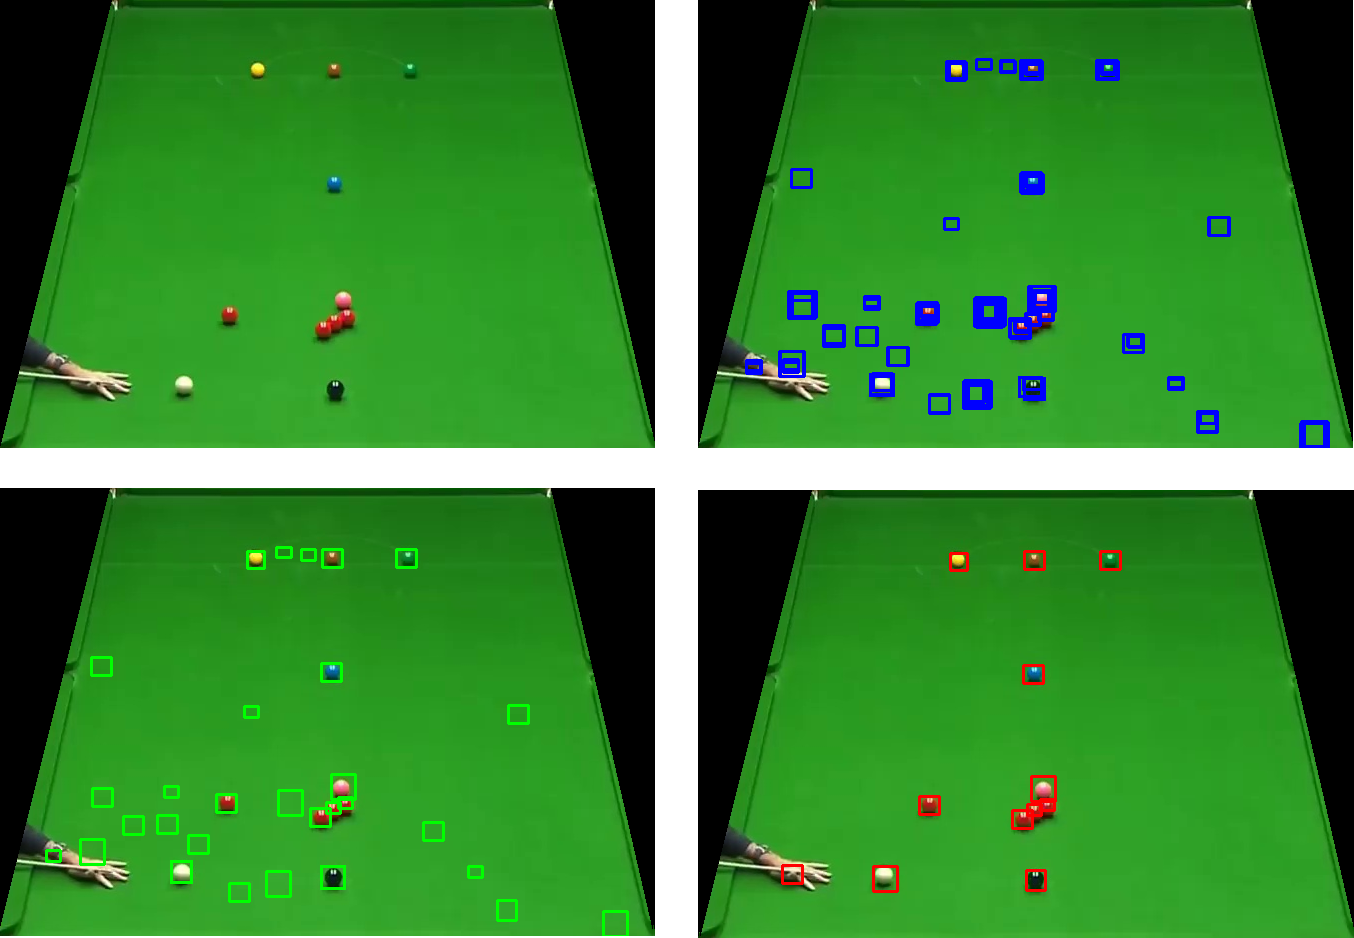
\includegraphics[scale=0.45]{1.png}
    \caption{Picture with snooker table after eliminating noise. Then with blue are the boxes 
    before non maxima fupression, with green after non maxima supression and with red after 
    eliminating the false positive.}   
    \label{fig:picture}
\end{figure}

A weighted voting system is used to determine the colors: each pixel in the exam patch provides 
a certain score for the color to which it belongs. Finally the color of the patch will be 
described by the most impactful 3 colors (the sum of the scores for each pixel in the examined 
patch) - the \emph{get\_box\_color} function. The final prediction is issued by the \emph{process\_colors} 
function which examines all the colors of the balls and changes the colors as follows: due 
to a series of false positive boxes to determine more black and white balls, which will be 
modified by the current function reducing everything to maximum 1. Then due to the great 
confusion between red, pink, yellow and brown there may be several pink balls for example. 
This is solved by transferring pink balls over 1 to red balls, etc. \textbf{The accuracy for color 
detection is 84\%.} \par

% %%%%%%%%%%%%%%%%%%%
\section*{Task 2}
% %%%%%%%%%%%%%%%%%%%

\emph{You receive a test set of 25 videos containing a player making a shot. In each
of the 25 videos the snooker table is seen from above. The task is to decide whether
a ball was potted into a pocket and if so recognize the color of the potted ball and
the pocket (one of the six pockets) where the ball was potted
(1 - top left corner, 2 - top right corner, 3 - bottom left corner, 4 - bottom right corner, 5
- middle left corner, 6 - middle right corner). 
In each of the 25 videos there will be a maximum of one ball being potted.}

To determine if a ball has been inserted in one of the 6 pockets, proceed as follows: determine the 
number of balls and their colors in the first frame but also in the N-10 frame (exactly as in task 
\# 1), if the preview video has N frames. Then if the number of balls in the last frame is less than 
the number in the first frame then the DA hypothesis is issued (ie a ball has been inserted). Of 
course occlusion brings problems in this approach. \par

If the hypothesis is YES, then the color is calculated immediately by examining the color dictionaries 
in the two frames. For the detection of the pocket, proceed as follows: the proximity (plus minus 90 
pixels) of the 6 pockets is analyzed throughout the video. If there is movement (the difference 
between frame i and frame i + 2 is more than 50 pixels that change) then I save the current frame 
for further analysis. This is done for all 6 pockets, resulting in 6 lists of frames in which there 
is movement in the area of ​​a pocket. In the end, the pocket is considered to be the one that has 
the maximum color score of the ball. Of course we work with normalized data (if in the list of pocket 
1 there are 5 frames and in the list of pocket 2 there are 80 frames then a score of the color of the 
ball that entered each of these frames is issued, it is added and is divided by their number). 
\textbf{The accuracy for this task is 88\%.} \par

% %%%%%%%%%%%%%%%%%%%
\section*{Task 3}
% %%%%%%%%%%%%%%%%%%%

\emph{you receive a test set of 25 videos containing a player making a shot. In
each of the 25 videos the snooker table is seen from above. The task is to track the
cue ball (the white ball) and another specified ball. The initial bounding boxes of the
two balls to be tracked are provided for the first frame (they follow the format [xmin
ymin xmax ymax], where (xmin,ymin) is the top left corner and (xmax,ymax) is the
bottom right corner of the initial bounding-box).
In each video we will consider that your algorithm correctly tracks a ball if in
more (greater or equal) than 80\% of the frames your algorithm correctly localizes the
ball to be tracked. We consider that your algorithm correctly localizes the ball to be
tracked in a specific frame if the value of the IOU (intersection over union) beetween
the window provided by your algorithm and the ground-truth window is more than 20\%. }

For this task we use CSRT tracker from OpenCV which for each frame in the image will issue a box containing 
the object of interest. Initially it receives as location what is read from the input file, then it will 
issue for each frame in the video a location of the ball of interest. The accuracy so far is very low, 
almost zero. Because if a ball goes into a pocket then the CSRT tracker will say that the ball is still 
in the pocket until the end of the video. \par

The essence of this task is the \emph{update\_boxes} function that will delete a series of boxes if a ball 
enters a pocket. This function receives as a parameter the video and the boxes given by the CSRT 
tracker. It calculates the areas of interest for the pockets (the center of the pocket plus minus 
75 pixels) then calculates the frame from which the analyzed ball starts to move, analyzing the 
frames from 5 to 5. If the intersection over union from frame i and at frame i-5 it is below 50\% then 
the ball is moving. Then to calculate the stopping point in motion, do the same - if the intersection 
over union at frame i and frame i-5 is 90\% then the ball does not move. In addition, if at this point 
the ball is on one of the areas of interest of the 6 pockets then it is considered that the ball 
has entered that pocket and the boxes at the end point of the movement are eliminated. In this way, 
\textbf{the accuracy for this task is 78\%.} \par

% %%%%%%%%%%%%%%%%%%%
\section*{(bonus) Task 4}
% %%%%%%%%%%%%%%%%%%%

\emph{You receive a test set of 25 videos containing a player making a
shot. Different than the previous tasks, in this videos the snooker table can be filmed
from different viewpoints (not only from above). The task is to track the cue ball.
The task here is much harder as you have diferent scales of the cue ball, changes in
camera viewpoint, the initial bounding box of the white ball is not provided. The
initial bounding box of the cue ball to be tracked is provided for the first frame (it
follows the format [xmin ymin xmax ymax], where (xmin,ymin) is the top left corner
and (xmax,ymax) is the bottom right corner of the initial bounding-box). 
The rules described at Task 3 apply here, meaning that your algorithm should correctly 
localizes the cue ball in more than 80\% of the frames, at each frame correctly localization
means that the window provided by your algorithm should have IOU more than 20\%
with respect to the ground-truth window.}

This task has not been addressed.

\end{document}